%!TEX root = MemoireZelliges.tex

\chapter{Étude physique d'un zellige vert (\bdx{6528})}
%======================================================================

\section{Description -- État de surface}
%----------------------------------------------------------------------

Cet échantillon, de forme parallélépipédique, est une pièce de 
céramique glaçurée de couleur verte (\fref{dessin:6528}). 
Il provient du \PaM (\siecle{17}) de Meknès. 
Il est chamfreiné. Les taches violacées sur la glaçure sont des 
traces d'encre dues à l'indexation de l'échantillon par les marocains.

\begin{itemize}
  \item \DimText : \SI{33x33x18}{\mm}
  \item \emph{Masse} : \SI{25.0}{\g}
\end{itemize}

\begin{figure}[htb]
  \begin{minipage}[t]{0.5\textwidth}
    \centerfloat
    \vspace*{0pt}
    % Dessin de l'échantillon : Vue de dessus
    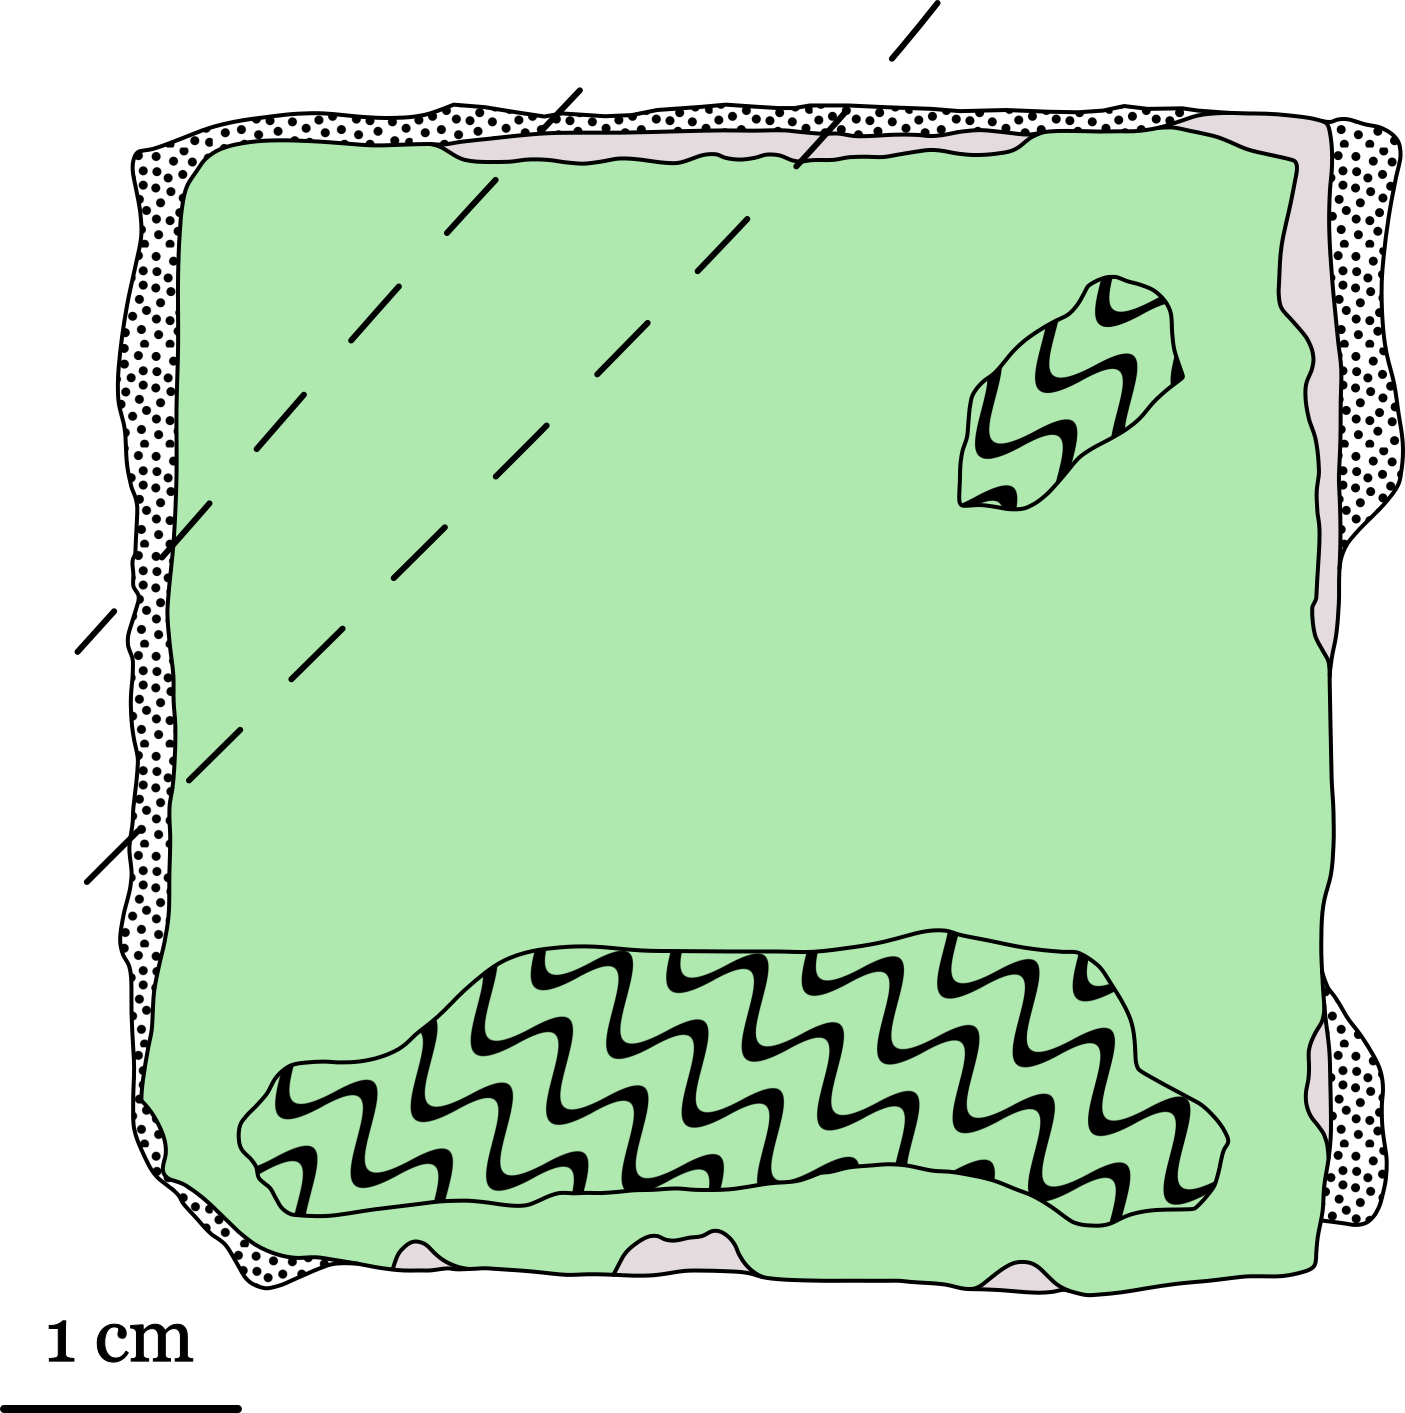
\includegraphics[scale=1]{PaM_BDX6528_dessus}
    \subcaption{Vue de dessus \label{dessin:6528_dessus}}
  \end{minipage}%
  \quad%
  \begin{minipage}[t]{0.5\textwidth}
    \centerfloat
    \vspace*{0pt}
    % Dessin de l'échantillon : Lame
    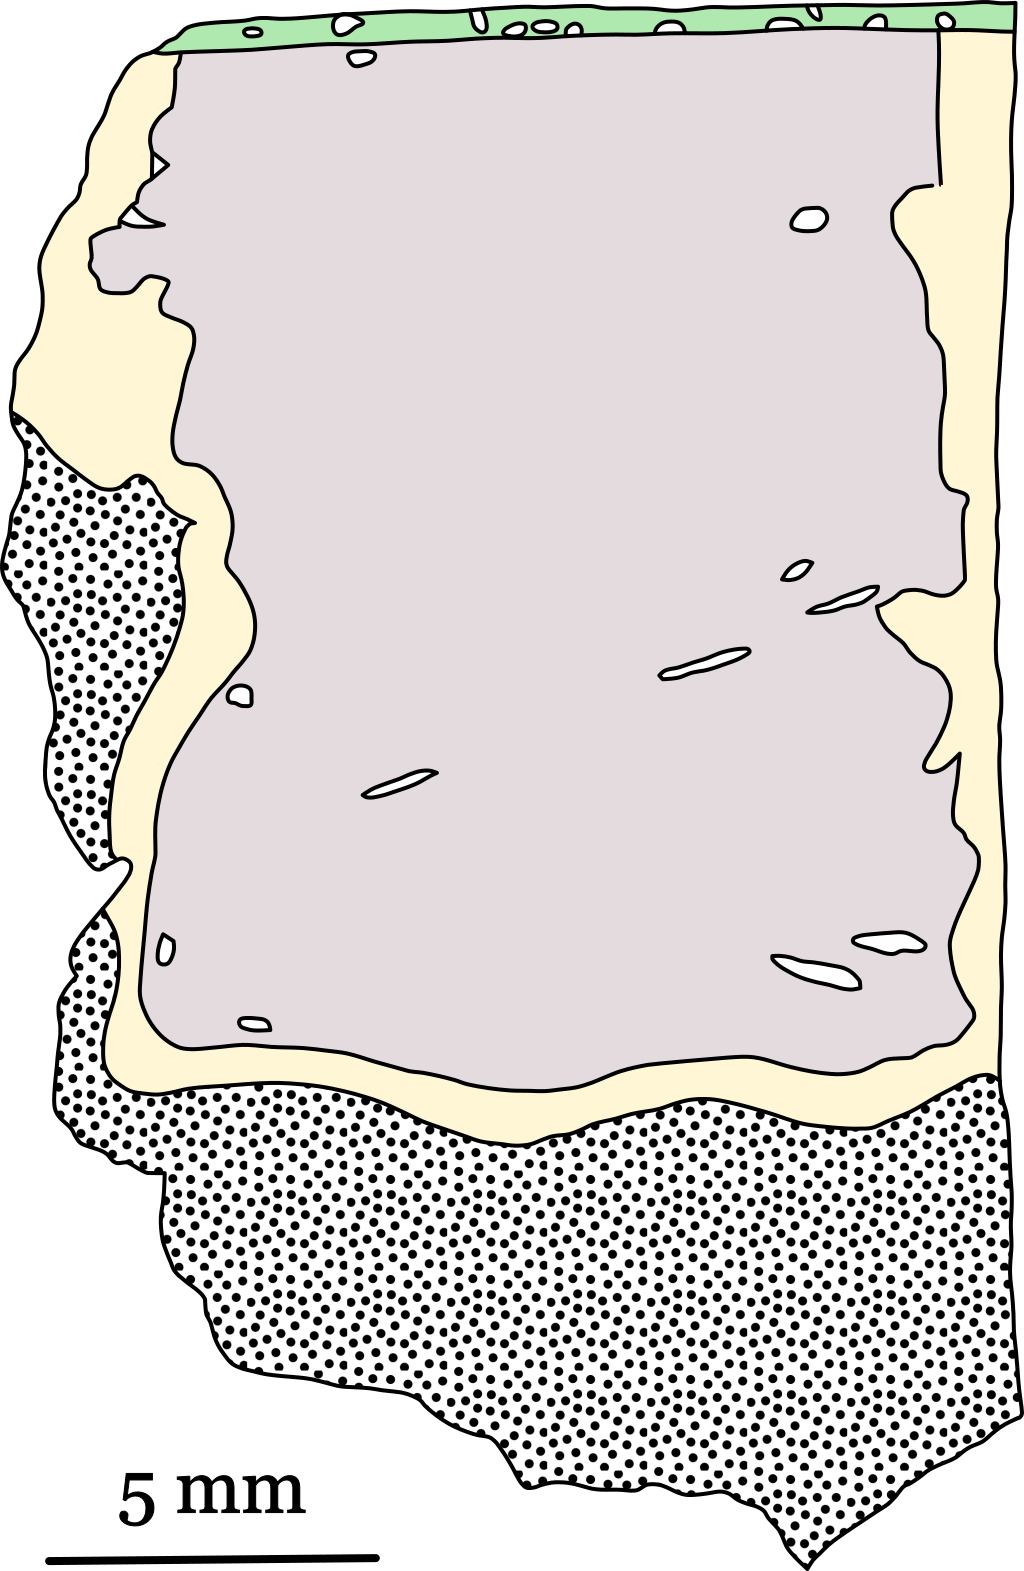
\includegraphics[scale=1]{PaM_BDX6528_lame}
    \subcaption{Lame étudiée \label{dessin:6528_lame}}
  \end{minipage}

  \bigskip

  \begin{minipage}[t]{0.5\textwidth}
    \centerfloat
    \vspace*{0pt}
    % Dessin de l'échantillon : Coupe
    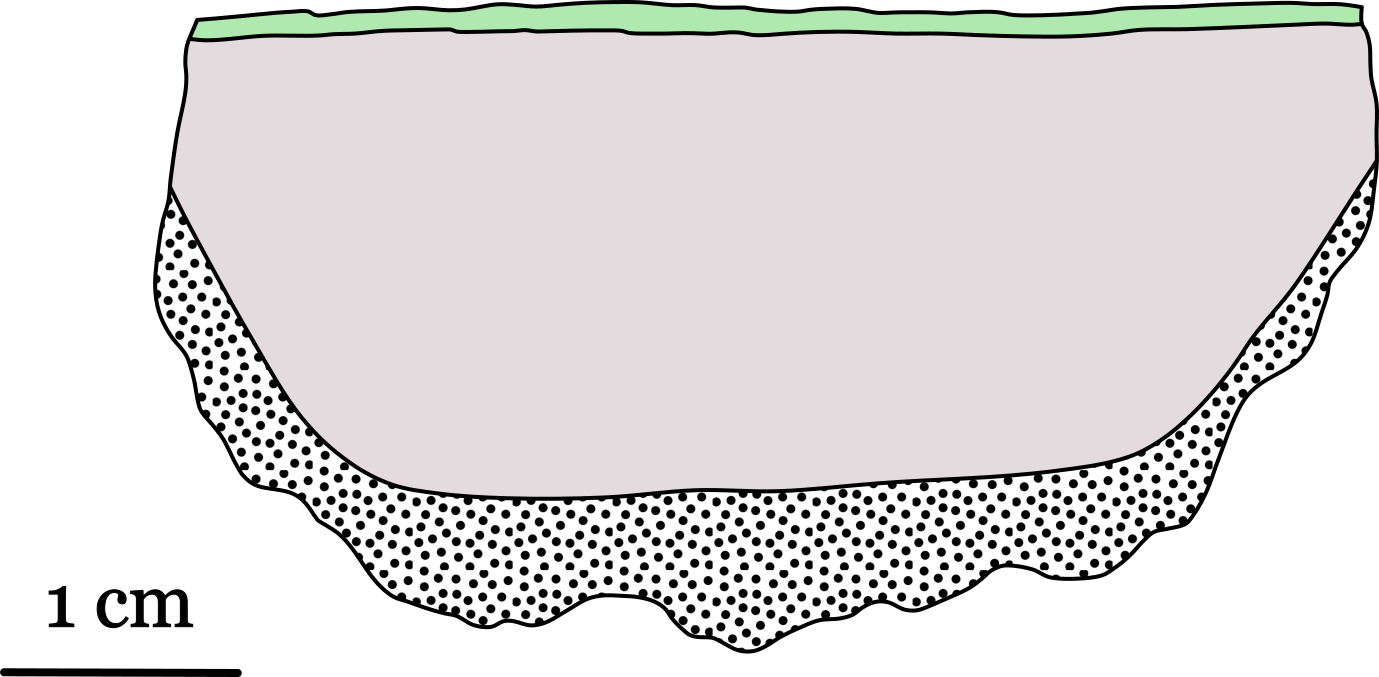
\includegraphics[scale=1]{PaM_BDX6528_coupe}
    \subcaption{Vue en coupe \label{dessin:6528_coupe}}
  \end{minipage}%
  \quad%
  \begin{minipage}[t]{0.5\textwidth}
    \vspace*{0pt}
    Légende :

    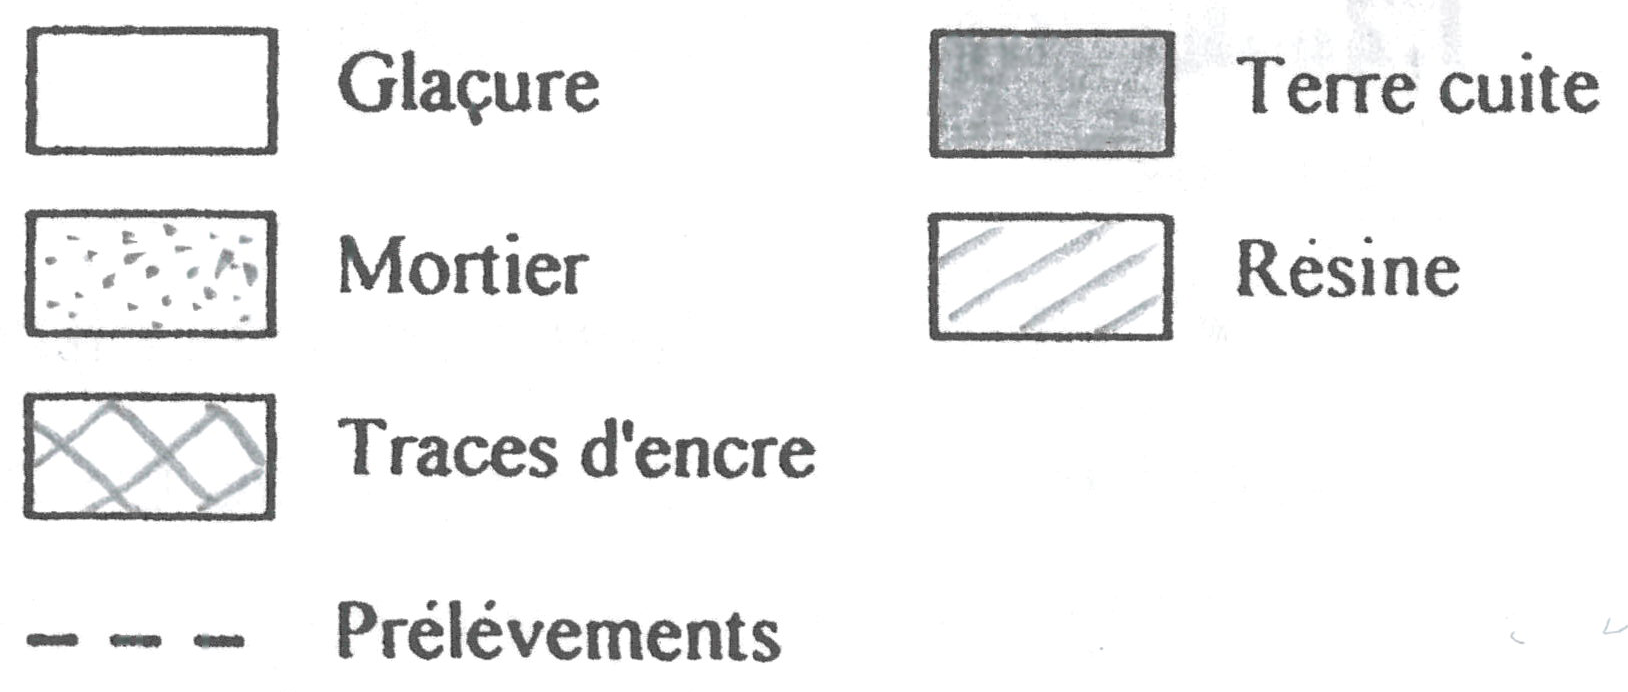
\includegraphics[scale=1]{dessin_legende}
    % \begin{itemize}
    %   \item Terre cuite
    %   \item Glaçure
    %   \item Résine
    %   \item Mortier
    %   \item Traces d'encre
    %   \item Prélévements
    % \end{itemize}
  \end{minipage}
  \caption[\bdx{6528}]{\legendeA 
           % a : vue de dessus, b : vue en coupe, c : lame étudiée.
          }
  \label{dessin:6528}
\end{figure}

L'observation de la surface de la glaçure (\fref{surf:6528}) montre 
qu'elle contient des bulles, des picots, présente des rayures et 
contient des cristaux non fondus. On peut aussi remarquer des taches 
blanches, dues peut-être à une cristallisation en surface ou à un 
piquetage du verre.

Le support de terre cuite est de couleur rougeâtre, de granulométrie 
fine, peu poreux et contient de nombreuses inclusions de tailles et 
de couleurs variées.

\begin{figure}[htb]
  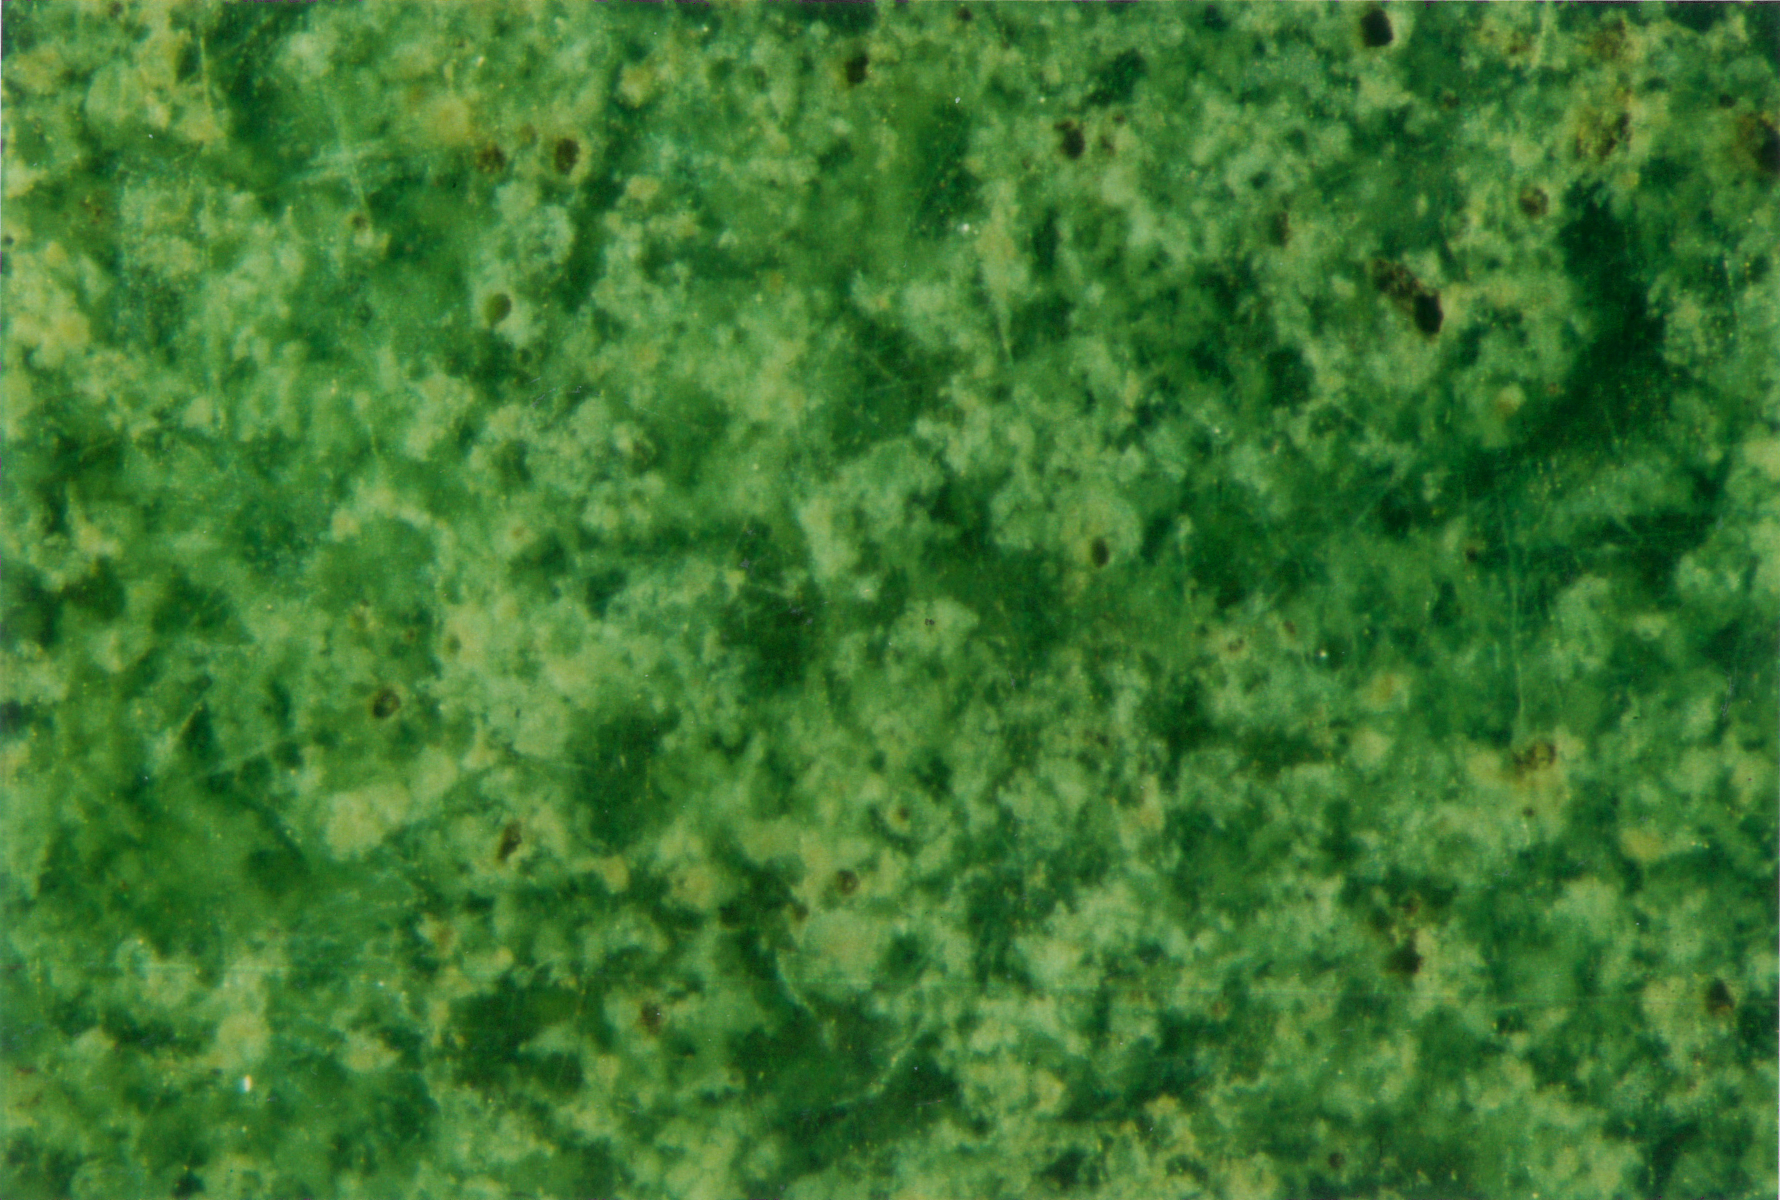
\includegraphics[width=\textwidth]{PaM_BDX6528_Surf}
  \caption[\bdx{6528}\ -- État de surface de la glaçure]
          {\legendeA 
           État de surface de la glaçure (Gr=30, \zone{\sim4.3x3.2}{\mm}). Elle contient des 
           bulles, des picots, des cristaux non fondus et présente 
           des rayures.}
  \label{surf:6528}
\end{figure}


\section{Étude de la couleur}
%----------------------------------------------------------------------

\subsection{Identification des ions chromogènes}
%~~~~~~~~~~~~~~~~~~~~~~~~~~~~~~~~~~~~~~~~~~~~~~~~~~~~~~~~~~~~~~~~~~~~~~
Le spectre d'\AO en mode réflexion diffuse de la glaçure verte 
(\fref{spectre:6528}) présente une bande d'absorption large commençant 
à \SI{550}{nm} et dont le maximum se situe vers \SI{795}{nm}. Cette 
absorption est attribuable au \ch{Cu^2+} \autocite{Lajarte_1979}. On 
peut également distinguer un épaulement vers \SI{440}{nm} et un autre 
vers \SI{380}{nm} correspondant au \ch{Fe^3+}. La glaçure étant 
transparente, il peut s'agir d'une contribution de la terre cuite 
qui présente, elle aussi, ces absorptions (\fref{spectre:6528}). 
La présence de \ch{Fe^3+} peut expliquer la teinte légèrement jaune 
du vert de la glaçure.

\begin{figure}[htb]
  \begin{plotspectre}
    \addplot [thick, PaleGreen!66!black] 
       table [x=lambda, y=6528gla] {\gladata} ;
    \addlegendentry{glaçure verte}
    \addplot [thick, FireBrick] 
       table [x=lambda, y=6528tc] {\tcdata} ;
    \addlegendentry{terre cuite}
  \end{plotspectre}
  \caption[\bdx{6528}\ -- Spectres d'\AO en mode réflexion diffuse 
           de la glaçure et de la terre cuite]
          {\legendeA.
           Spectres d'\AO en mode réflexion diffuse de la glaçure et 
           de la terre cuite. La coloration verte de la glaçure est 
           due au \ch{Cu^2+} mis en évidence par la bande large à 
           partir de \SI{550}{\nm}. Le spectre de la terre cuite 
           présente deux bandes à \SIlist{380;440}{\nm}, attribuables 
           au \ch{Fe^3+} \autocite{Lajarte_1979}.}
  \label{spectre:6528}
\end{figure}

\subsection{Mesure physique de la couleur}
%~~~~~~~~~~~~~~~~~~~~~~~~~~~~~~~~~~~~~~~~~~~~~~~~~~~~~~~~~~~~~~~~~~~~~~
Les coordonnées \trichros correspondant aux espaces \Yxy et \Lab 
ont été obtenues à partir du spectre d'\AO{} (\tref{saotab:6528}). 
La longueur d'onde dominante obtenue pour la glaçure la place dans 
le domaine des vert-jaune \autocite{Kelly_1976}. La relativement 
faible réflectance $Y$ révèle une couleur assez foncée et la 
pureté d'excitation est celle d'une couleur peu saturée. La
\fref{colorfig:6528} présente la localisation des coordonnées 
chromatiques de la glaçure verte dans les espaces \Yxy et \Lab. 
La terre cuite a une longueur d'onde dominante de \SI{580.75}{\nm} 
qui la situe dans le domaine du jaune orange.

\begin{table}
  \begin{chrotab}
      \chrolgna{Glaçure}{563.41}{20.39}
               {28.102}{0.330}{0.384}
               {59.981}{-10.927}{15.673} &
      \chrolgnb{vert jaune foncé}{Vert-Jaune}{560}{570}
               {\footnotemark{}}
    \tabularnewline
      \chrolgna{Terre cuite}{580.75}{21.53}
               {47.846}{0.357}{0.362}
               {74.728}{4.772}{16.629} &
      \chrolgnb{jaune orange clair}{Jaune-Orange}{580}{585}
               {\footnotemark{}}
    \tabularnewline
  \end{chrotab}
  \caption[\bdx{6528}\ -- Coordonnées chromatiques et longueur d'onde 
           dominante]
          {\legendeA 
           Coordonnées chromatiques dans les systèmes \Yxy et \Lab 
           et longueur d'onde dominante (illuminant D65, \ang{2},
           \SIrange{400}{700}{\nm}).}
  \label{saotab:6528}
\end{table}
% \begin{table}
%   \begin{saotab}
%       \saolgna{Glaçure}{563.41}{20.39}
%               {28.102}{0.330}{0.384}
%               {59.981}{-10.927}{15.673} &
%       \saolgnb{vert jaune foncé}{Vert-Jaune}{560}{570}
%               {\footnotemark{}}
%     \tabularnewline
%       \saolgna{Terre cuite}{580.75}{21.53}
%               {47.846}{0.357}{0.362}
%               {74.728}{4.772}{16.629} &
%       \saolgnb{jaune orange clair}{Jaune-Orange}{580}{585}
%               {\footnotemark{}}
%     \tabularnewline
%   \end{saotab}
%   \caption[\bdx{6528}\ -- Coordonnées chromatiques et longueur d'onde 
%            dominante]
%           {\legendeA 
%            Coordonnées chromatiques dans les systèmes \Yxy et \Lab 
%            et longueur d'onde dominante (illuminant D65, \ang{2},
%            \SIrange{400}{700}{\nm}).}
%   \label{saotab:6528}
% \end{table}
\footnotetext{\autocite{Kelly_1976}}
\footnotetext{\autocite{Kelly_1976}}

\begin{figure}[htb]
  \newcommand{\samplename}{6528gla}
  \newcommand{\samplecolor}{PaleGreen}
  \begin{minipage}[t]{0.37\paperwidth}
    \begin{plotYxy}
      \plotYxyPaV ;
      \plotYxyIlluminant ;
      \plotYxySample{\samplename}{\samplecolor} ;
      \plotYxyLigne{\samplename} ;
      \plotYxyAnnot{\samplename}{south west} ;
    \end{plotYxy}
    \subcaption{espace \trichro \Yxy. La longueur d'onde 
                dominante de la glaçure est \SI{563.413}{\nm}. 
                Elle est dans le domaine de vert-jaune. Le point 
                représentatif est proche de l'illuminant standard, 
                la couleur est peu saturée.}
  \end{minipage}%
  \qquad%
  \begin{minipage}[t]{0.37\paperwidth}
    \begin{plotLab}
      \plotLabSample{\samplename}{\samplecolor} ;
    \end{plotLab}
    \subcaption{espace \trichro \Lab. Le point représentatif 
                de la couleur de la glaçure est dans le quart 
                vert-jaune.}
  \end{minipage}%
  \caption[\bdx{6528}\ -- Espaces \trichros]
          {\legendeA Analyse chromamétrique de la glaçure.}
  \label{colorfig:6528}
\end{figure}


\section{Étude de la texture de la glaçure et de la terre cuite sur 
         une section polie}
%----------------------------------------------------------------------

\subsection{Observation en lumière naturelle}
%~~~~~~~~~~~~~~~~~~~~~~~~~~~~~~~~~~~~~~~~~~~~~~~~~~~~~~~~~~~~~~~~~~~~~~
\begin{figure}[htb]
  \begin{minipage}[t]{0.4\textwidth}
    \fakeimg{lum. nat.}
    \subcaption{Lumière naturelle \label{texture:6528_LN}}
  \end{minipage}
  \begin{minipage}[t]{0.4\textwidth}
    \fakeimg{Cathodo}
    \subcaption{\CL \label{texture:6528_CL}}
  \end{minipage}
  \caption[\bdx{6528}\ -- Observation de la texture en section]
          {\legendeA 
           Observation de la texture en section sur une surface de 
           \SI{2.6x1.9}{\mm}.}
  \label{texture:6528}
\end{figure}

L'examen d'une section en lumière naturelle 
(\fref{texture:6528_LN}) montre que la glaçure est colorée dans 
la masse et qu'elle adhère bien au support de terre cuite. La terre 
cuite contient de nombreuses inclusions de tailles et de couleurs 
diverses, réparties de manière homogène.

La limite entre la glaçure et le support de céramique semble 
particulièrement nette.

\subsection{Observation en \CL}
%~~~~~~~~~~~~~~~~~~~~~~~~~~~~~~~~~~~~~~~~~~~~~~~~~~~~~~~~~~~~~~~~~~~~~~
La glaçure n'est pas luminescente (\fref{texture:6528_CL}).

La terre cuite présente une luminescence mauve et contient des 
inclusions qui luminescent en rouge ou bleu, réparties de manière 
homogène dans l'ensemble du matériau.

À l'interface terre cuite-glaçure, on observe un très faible liseré 
qui luminescence en bleu.

\subsection{Observation en \MEB[ie]}
%~~~~~~~~~~~~~~~~~~~~~~~~~~~~~~~~~~~~~~~~~~~~~~~~~~~~~~~~~~~~~~~~~~~~~~
La glaçure a une épaisseur moyenne de \SI{350}{\um}. Elle contient des 
bulles. On peut également distinguer des cristaux de néoformation dans 
sa masse et à l'interface glaçure-terre cuite 
(\fref{MEB:6528_img}).

Une \carto de \RX (\fref{MEB:6528_carto_tcgla}) a permis de distinguer la présence de cristaux non fondus de quartz dans la glaçure. Celle-ci est également riche en plomb et contient du cuivre. Elle est en revanche moins riche en calcium et aluminium que la terre cuite.

\begin{figure}[htb]
  \fakeimg{Texture au MEB, retrodiff (fig 23)}
  \caption[\bdx{6528}\ -- Observation de la texture au \MEB, 
           en mode \ERD. Ensemble glaçure/terre cuite]
          {\legendeA
           Observation de la texture au \MEB, en mode \ERD. 
           Ensemble glaçure/terre cuite. La barre d'échelle mesure 
           \SI{200}{\um} (\zone{650x530}{\um}).}
  \label{MEB:6528_img}
\end{figure}

L'interface glaçure-terre cuite semble être riche en potassium et 
calcium. Son faible développement laisse supposer des interactions 
faibles entre ces deux matériaux  et peut donc faire envisager 
l'hypothèse d'une application de la glaçure sur une terre cuite.

La terre cuite contient des inclusions (\SIrange[range-phrase=\ à\ ]{50}{150}{\um}), identifiées par \carto de \RX (\fref{MEB:6528_carto_tc}), comme des cristaux de quartz et de feldspaths potassiques et sodiques. La présence de ces derniers peut être corrélée avec les luminescences ponctuelles bleues détectées en \CL. Le calcium présent dans toute la terre cuite peut être responsable, sous forme de calcite, des luminescences rouges détectées en \CL.

\noindent Remarque : le mauvais état de surface de la lame est dû aux 
contraintes mécaniques qu'elle subit lors du sciage et du polissage.

\begin{figure}[htb]
  \fakeimg{Texture au MEB, carto tc/gla (fig 24)}
  \caption[\bdx{6528}\ -- Observation de la texture au \MEB, \carto de \RX de l'ensemble glaçure/terre cuite]
          {\legendeA
           Observation de la texture au \MEB, \carto de \RX de l'ensemble glaçure/terre cuite (Gr=150, \zone{735x600}{\um}).}
  \label{MEB:6528_carto_tcgla}
\end{figure}

\begin{figure}[htb]
  \fakeimg{Texture au MEB, carto tc (fig 25)}
  \caption[\bdx{6528}\ -- Observation de la texture au \MEB, \carto de \RX de la terre cuite]
          {\legendeA
           Observation de la texture au \MEB, \carto de \RX de la terre cuite (Gr=190, \zone{580x475}{\um}).}
  \label{MEB:6528_carto_tc}
\end{figure}


\section{Composition élémentaire de la glaçure}
%----------------------------------------------------------------------

\begin{table}
  \begin{cartotab}
    % \toprule
      \cartolgn{SiO2}{36.55}{3.79} &
      \cartolgn{CaO}{2.43}{0.23}   &
      \cartolgn{Al2O3}{2.37}{0.18} &
      \cartolgn{MgO}{0.67}{0.08}
    \tabularnewline
      \cartolgn{Na2O}{0.34}{0.02}  &
      \cartolgn{K2O}{0.91}{0.10}   &
      \cartolgn{Fe2O3}{1.13}{0.09} &
      \cartolgn{PbO}{54.49}{4.05}
    \tabularnewline
      \cartolgnnd{SnO2}          &
      \cartolgn{CuO}{0.72}{0.09} &
      \cartolgnnd{CoO}           &
      \cartolgnnd{MnO}
    \tabularnewline
      \cartolgnnd{Cr2O3} &
      \cartolgnnd{ZnO}   &
      \cartolgnnd{Sb2O3} &
      \cartolgn{TiO2}{0.15}{0.06}
    \tabularnewline
      \cartolgnnd{S}            &
      \cartolgnnd{P2O5}         &
      \cartolgn{Cl}{0.25}{0.05} &
      \cartolgnnd{As2O3}
    \tabularnewline
    % \midrule
    %   \cartolgntt
    % \bottomrule
  \end{cartotab}
  \caption[\bdx{6528}\ -- Analyse quantitative par \EDS, composition 
           élémentaire de la glaçure]
          {\legendeA Analyse quantitative par \EDS. Composition 
           élémentaire de la glaçure verte sur une surface de 
           \SI{108x88}{\um} (\PMO).}
  \label{compelem:6528_gla}
\end{table}

Le \tref{compelem:6528_gla} présente la composition élémentaire 
de la glaçure blanche obtenue par \EDS. Ils sont donnés en pourcentages massiques d'oxyde normalisés à \SI{100}{\percent}. Ce sont des moyennes de trois à cinq mesures effectuées sur toute la longueur de la glaçure, sur la zone d'analyse la plus grande possible, et en prenant garde d'éviter les bulles et cristaux non fondus. Il en est de même pour toutes les compositions élémentaires présentées dans ce mémoire.

Il s'agit d'une glaçure plombifère transparente. La présence de 
cuivre (\SI{0.72}{\percent} de \ch{CuO}), détecté également en \SAO 
sous la forme \ch{Cu^2+}, est responsable de sa couleur verte. Elle 
est très légèrement teintée de jaune, probablement à cause de la 
présence de \ch{Fe^3+} (\SI{1.13}{\percent} de \ch{Fe2O3}).


\section{Étude de la terre cuite support}
%----------------------------------------------------------------------

\subsection{Composition élémentaire}
%~~~~~~~~~~~~~~~~~~~~~~~~~~~~~~~~~~~~~~~~~~~~~~~~~~~~~~~~~~~~~~~~~~~~~~
Comme pour la glaçure, les résultats sont présentés en pourcentages 
massiques d'oxyde et sont des moyennes de trois à cinq mesures 
réparties dans l'ensemble de la terre cuite (\tref{compelem:6528_tc}).

La terre cuite est riche en calcium (\SI{20.30}{\percent} 
de \ch{CaO}). Sa coloration ocre rosé est due au \ch{Fe^3+} 
(\SI{7.18}{\percent} de \ch{Fe2O3}) en atmosphère de cuisson 
oxydante \autocite{Echallier_1984}.

\begin{table}
  \begin{cartotab}
      \cartolgn{SiO2}{53.71}{2.42} &
      \cartolgn{CaO}{20.30}{1.22} &
      \cartolgn{Al2O3}{12.58}{0.68} &
      \cartolgn{MgO}{3.10}{0.24}
    \tabularnewline
      \cartolgn{Na2O}{0.63}{0.05} &
      \cartolgn{K2O}{1.53}{0.07} &
      \cartolgn{Fe2O3}{7.18}{0.65} &
      \cartolgnnd{PbO} 
    \tabularnewline
      \cartolgnnd{SnO2} &
      \cartolgnnd{CuO} &
      \cartolgnnd{CoO} &
      \cartolgnnd{MnO} 
    \tabularnewline
      \cartolgnnd{Cr2O3} &
      \cartolgnnd{ZnO} &
      \cartolgnnd{Sb2O3} &
      \cartolgn{TiO2}{0.68}{0.04}
    \tabularnewline
      \cartolgn{S}{0.19}{0.03} &
      \cartolgnnd{P2O5} &
      \cartolgn{Cl}{0.09}{0.02} &
      \cartolgnnd{As2O5} 
    \tabularnewline
  \end{cartotab}
  \caption[\bdx{6528}\ -- Analyse quantitative par \EDS, composition élémentaire de la terre cuite]
          {\legendeA Analyse quantitative par \EDS. Composition élémentaire de la terre cuite sur une surface de \SI{2160x1752}{\um} (\PMO).}
  \label{compelem:6528_tc}
\end{table}

La présence de calcium dans une argile favorise l'attaque, à haute 
température, des silicates pour former des phases telles que la 
gehlénite ou le diopside. La gehlénite peut piéger les ions ferreux 
ou ferriques et empêcher ainsi la formation, en atmosphère oxydante, 
de l'hématite (\ch{Fe2O3}) qui donne à la céramique sa coloration 
plus ou moins rouge. Ici, on peut supposer que tout le fer présent 
dans l'argile de départ n'a pas été piégé par les phases haute 
température et que cet excès est responsable de la coloration de 
la terre cuite.

\subsection{Composition \cristallo}
%~~~~~~~~~~~~~~~~~~~~~~~~~~~~~~~~~~~~~~~~~~~~~~~~~~~~~~~~~~~~~~~~~~~~~~
\begin{figure}[htb]
  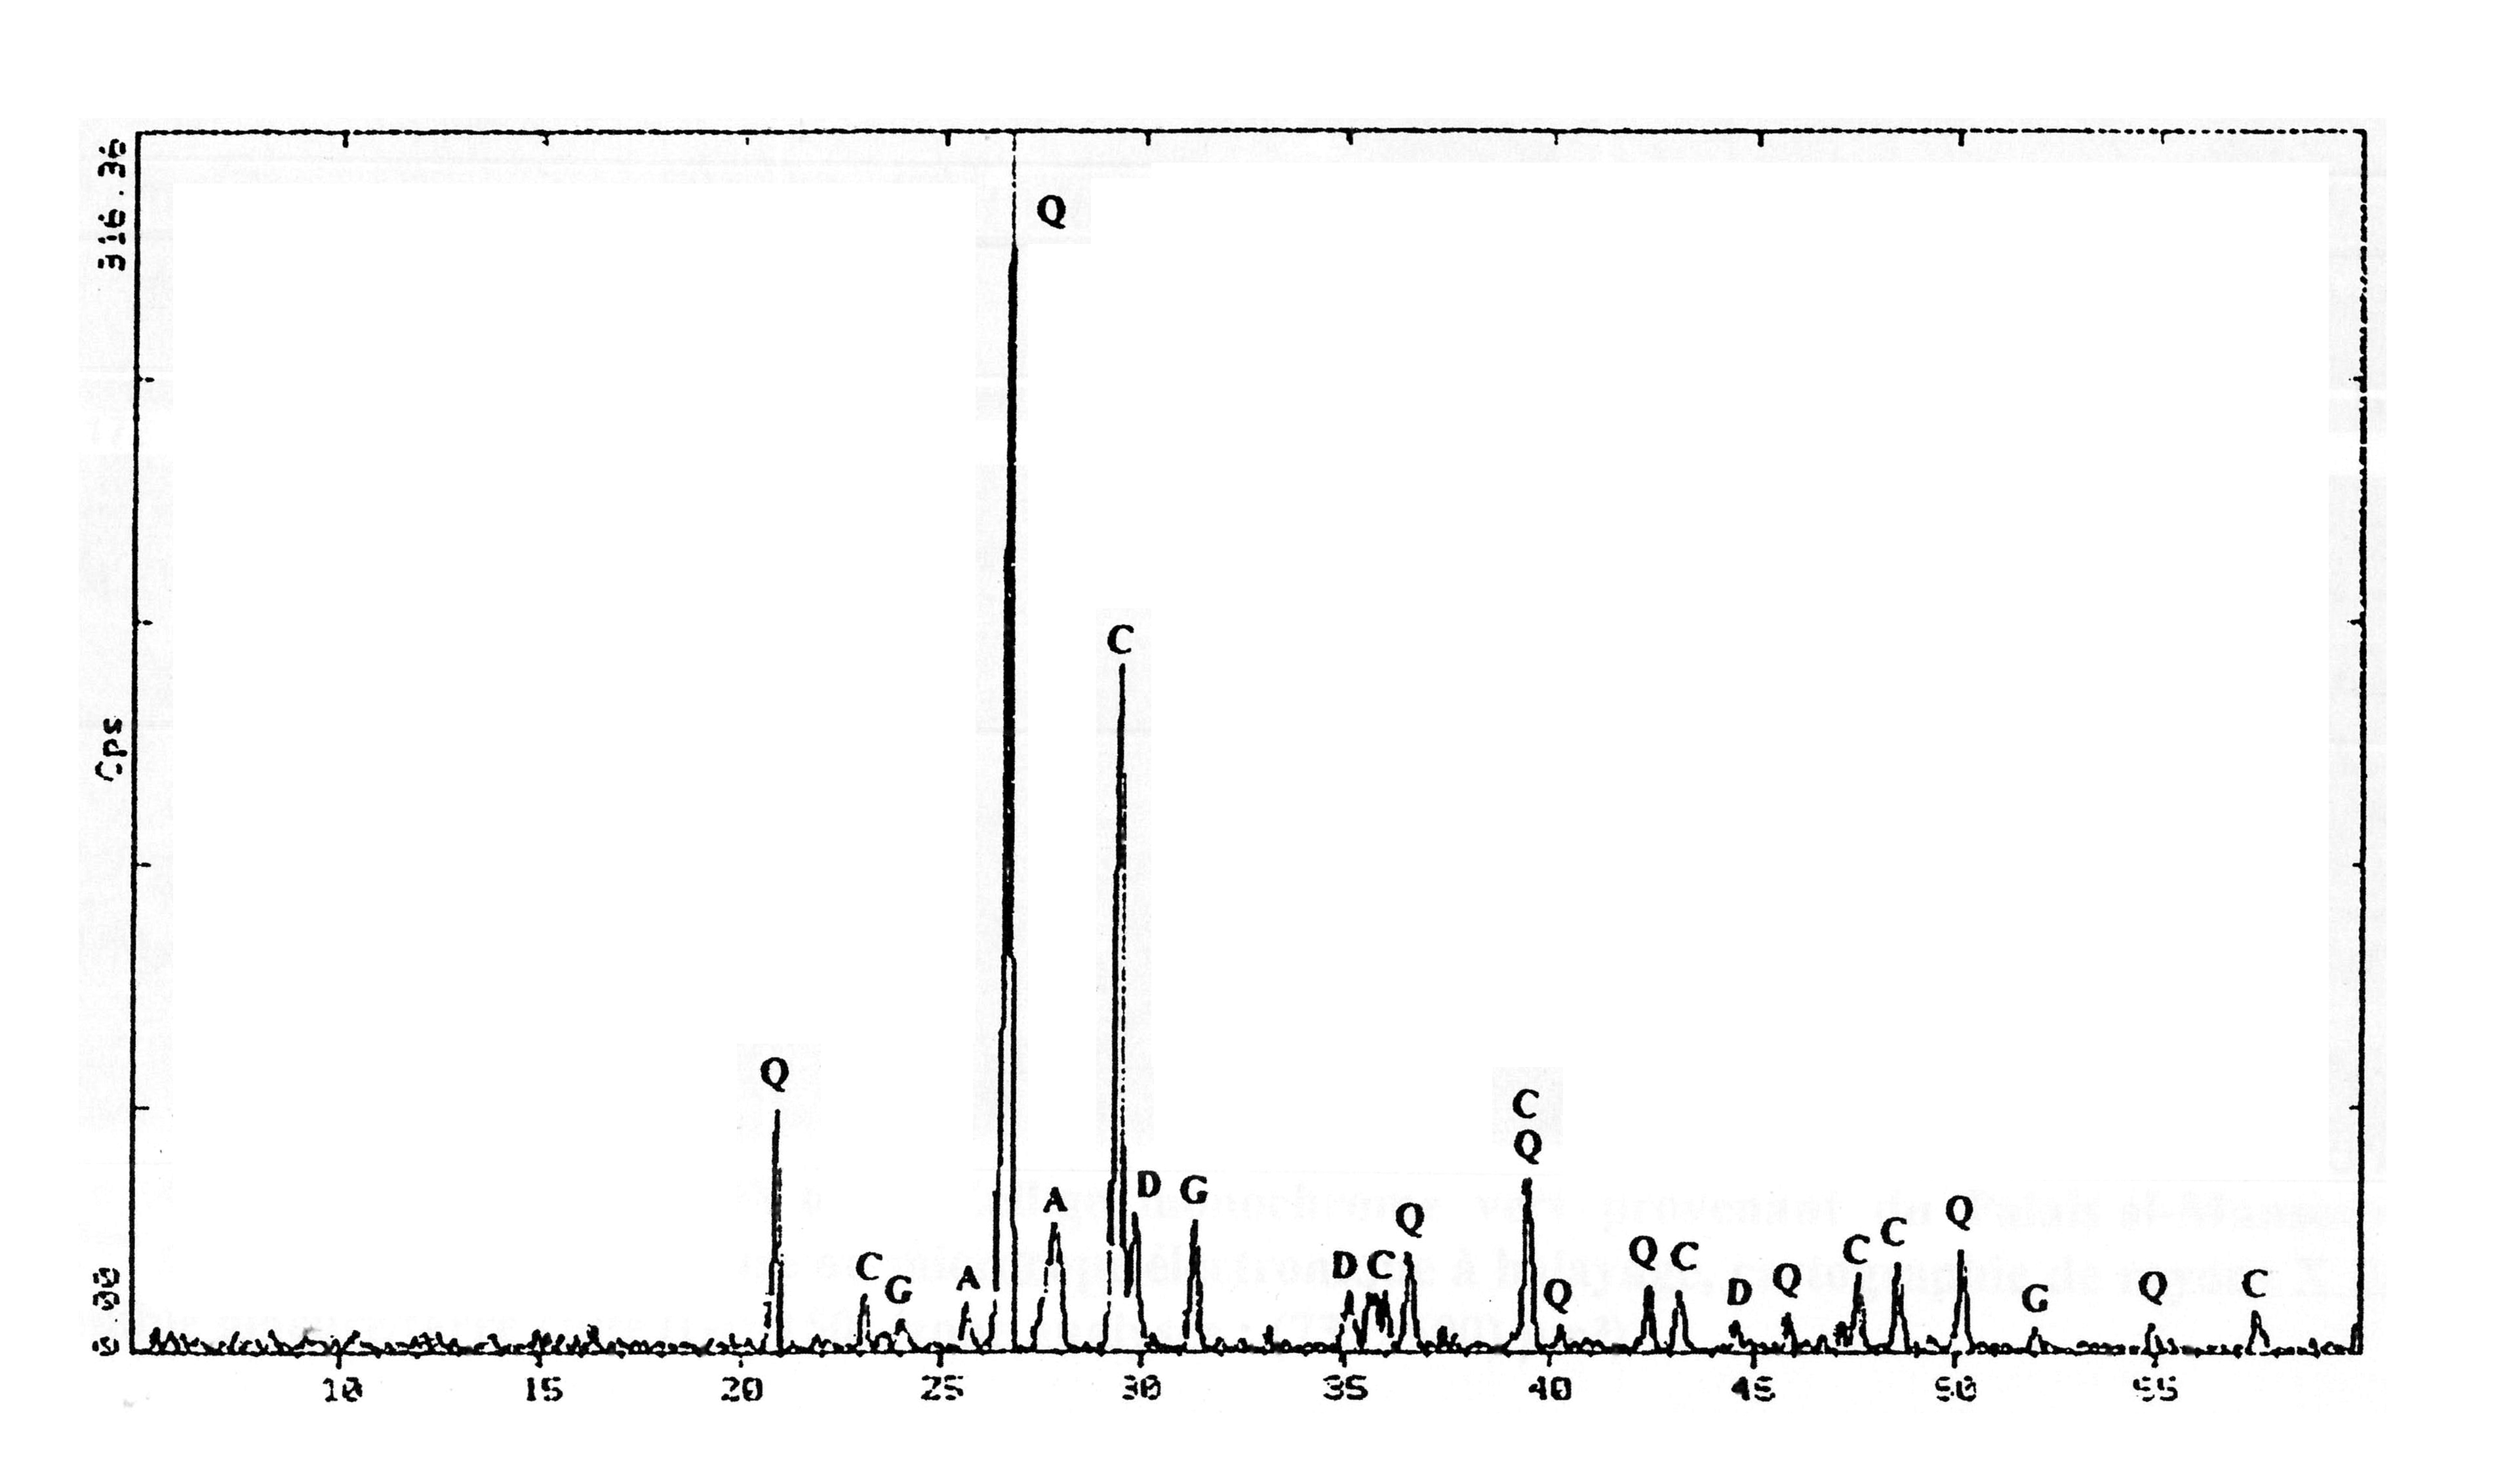
\includegraphics[width=\textwidth]{PaM_BDX6528_DX}
  \caption[\bdx{6528}\ -- \DX sur poudre de la terre cuite]
          {\legendeA 
           \DX sur poudre de la terre cuite. Mise en évidence de la présence de quartz (Q), calcite (C), gehlénite (G), anorthite (A), diopside (D).}
  \label{DRX:6528}
\end{figure}

La principale phase cristalline mise en évidence par \DX sur 
poudre (\fref{DRX:6528}) est le quartz (\quartz), responsable de la 
luminescence mauve de la terre cuite. On note également la présence de 
calcite (\calcite) qui peut être associée aux luminescences rouges 
détectées en \CL. Enfin, La terre cuite contient également des phases 
haute température telles que le diopside alumineux (\diopsidealfe), la 
gehlénite (\gehlenite) et l'anorthite (\anorthite). Les luminescences 
bleues détectées en \CL peuvent être associées à la présence de 
diopside et de géhlénite.

La présence de ces phases haute température laisse penser 
que la température de cuisson de la terre cuite aurait atteint 
\SIrange[range-phrase=\ à\ ]{900}{950}{\degC}.


\section{Sur la présence et l'identification de cristaux de 
         dévitrification}
%----------------------------------------------------------------------

On distingue, dans la masse de la glaçure et dans la zone d'interface entre celle-ci et la terre cuite, des cristaux de forme polygonale (\fref{MEB:6528_img_cx}). Ce sont des cristaux de dévitrification. Ils se développent pendant le refroidissement lent de la glaçure à partir de germes formés à haute température. Des analyses ponctuelles (\tref{compelem:6528_cx}) et une \carto de \RX ont montré qu'il s'agit de silicates de magnésium et de calcium.

\begin{figure}[htb]
  \fakeimg{6528ER96}
  \caption[\bdx{6528}\ -- Image en mode \ERD, cristaux de 
           dévitrification de forme polygonale]
          {\legendeA 
           Observation au \MEB, image en mode \ERD. Cristaux de 
           dévitrification de forme polygonale. La barre d'échelle 
           mesure \SI{10}{\um} \zone{33x27}{\um}.}
  \label{MEB:6528_img_cx}
\end{figure}

\begin{table}
  \begin{cartotab}
    % \toprule
      \cartolgn{SiO2}{50.12}{3.37} &
      \cartolgn{CaO}{16.80}{2.58}  &
      \cartolgn{Al2O3}{2.73}{1.39} &
      \cartolgn{MgO}{21.95}{3.09}
    \tabularnewline
      \cartolgnnd{As2O5} &
      \cartolgnnd{Na2O}  &
      \cartolgnnd{K2O}   &
      \cartolgn{Fe2O3}{3.94}{2.24} 
    \tabularnewline
      \cartolgn{PbO}{3.88}{0.90} &
      \cartolgnnd{SnO2} &
      \cartolgn{CuO}{0.30}{0.23} &
      \cartolgnnd{CoO}
    \tabularnewline
      \cartolgnnd{MnO} &
      \cartolgnnd{Cr2O3} &
      \cartolgnnd{ZnO} &
      \cartolgnnd{Sb2O3}
    \tabularnewline
      \cartolgn{TiO2}{0.23}{0.07} &
      \cartolgn{S}{0.12}{0.04} &
      \cartolgnnd{P2O5} &
      \cartolgnnd{Cl}
    \tabularnewline
    % \cartolgntt
  \end{cartotab}
  \caption[\bdx{6528}\ -- Analyse quantitative par \EDS, composition élémentaire des cristaux de dévitrification]
          {\legendeA Analyse quantitative par \EDS. Composition élémentaire des cristaux de dévitrification par analyses ponctuelles (\SI{1}{\um\squared}) (\PMO).}
  \label{compelem:6528_cx}
\end{table}

Ces analyses élémentaires doivent être considérées avec prudence : 
en effet, les faibles dimensions de ces cristaux 
(\SIrange[range-phrase=\ à\ ]{1}{2}{\um} dans leur plus petite 
dimension) ne permettent pas de certifier que la glaçure avoisinante 
n'entre pas en compte dans les analyses.


\section{Étude des altérations de la glaçure}
%----------------------------------------------------------------------

Aucune figure d'altération n'a été mise en évidence dans la glaçure, 
ni visuellement, ni en \MEB[ie] (MEB).


\section{Bilan}
%----------------------------------------------------------------------

Cet échantillon est donc une pièce de céramique portant une 
glaçure plombifère dont la coloration verte est due au \ch{Cu^2+} 
en atmosphère de cuisson oxydante.

Son support de terre cuite est de type calcique. Sa coloration 
ocre-rose est due à la présence de \ch{Fe^3+} en atmosphère de 
cuisson oxydante.

Sa composition \cristallo (quartz, calcite, diopside, 
gehlénite, anorthite) laisse penser qu'elle a été cuite à une 
température de l'ordre de 
\SIrange[range-phrase=\ à\ ]{900}{950}{\degC}.

A l'interface glaçure-terre cuite, on distingue un très fin liseré 
présentant une luminescence bleue, associé à la présence de cristaux 
de dévitrification identifiés comme des silicates de magnésium et de 
calcium. Le faible développement de cette zone laisse envisager 
l'application du mélange glaçurant sur une terre cuite.

La glaçure ne présente pas de figure d'altération d'origine chimique 
mais une usure mécanique de surface.
